\section{Estudo de caso}
\subsection{Processo industrial de manufatura}
A Fig. \ref{fig:processo} apresenta uma simulação para a planta industrial.
A composição da planta é a seguinte:
\begin{itemize}
    \item Tartaruga de entrega de peças;
    \item Mesa centralizadora com teste de chapa dupla;
    \item 5 robôs manipuladores;
    \item 4 prensas;
    \item Esteira para destinação final das peças;
\end{itemize}

\begin{figure}[H]%
    \centering
    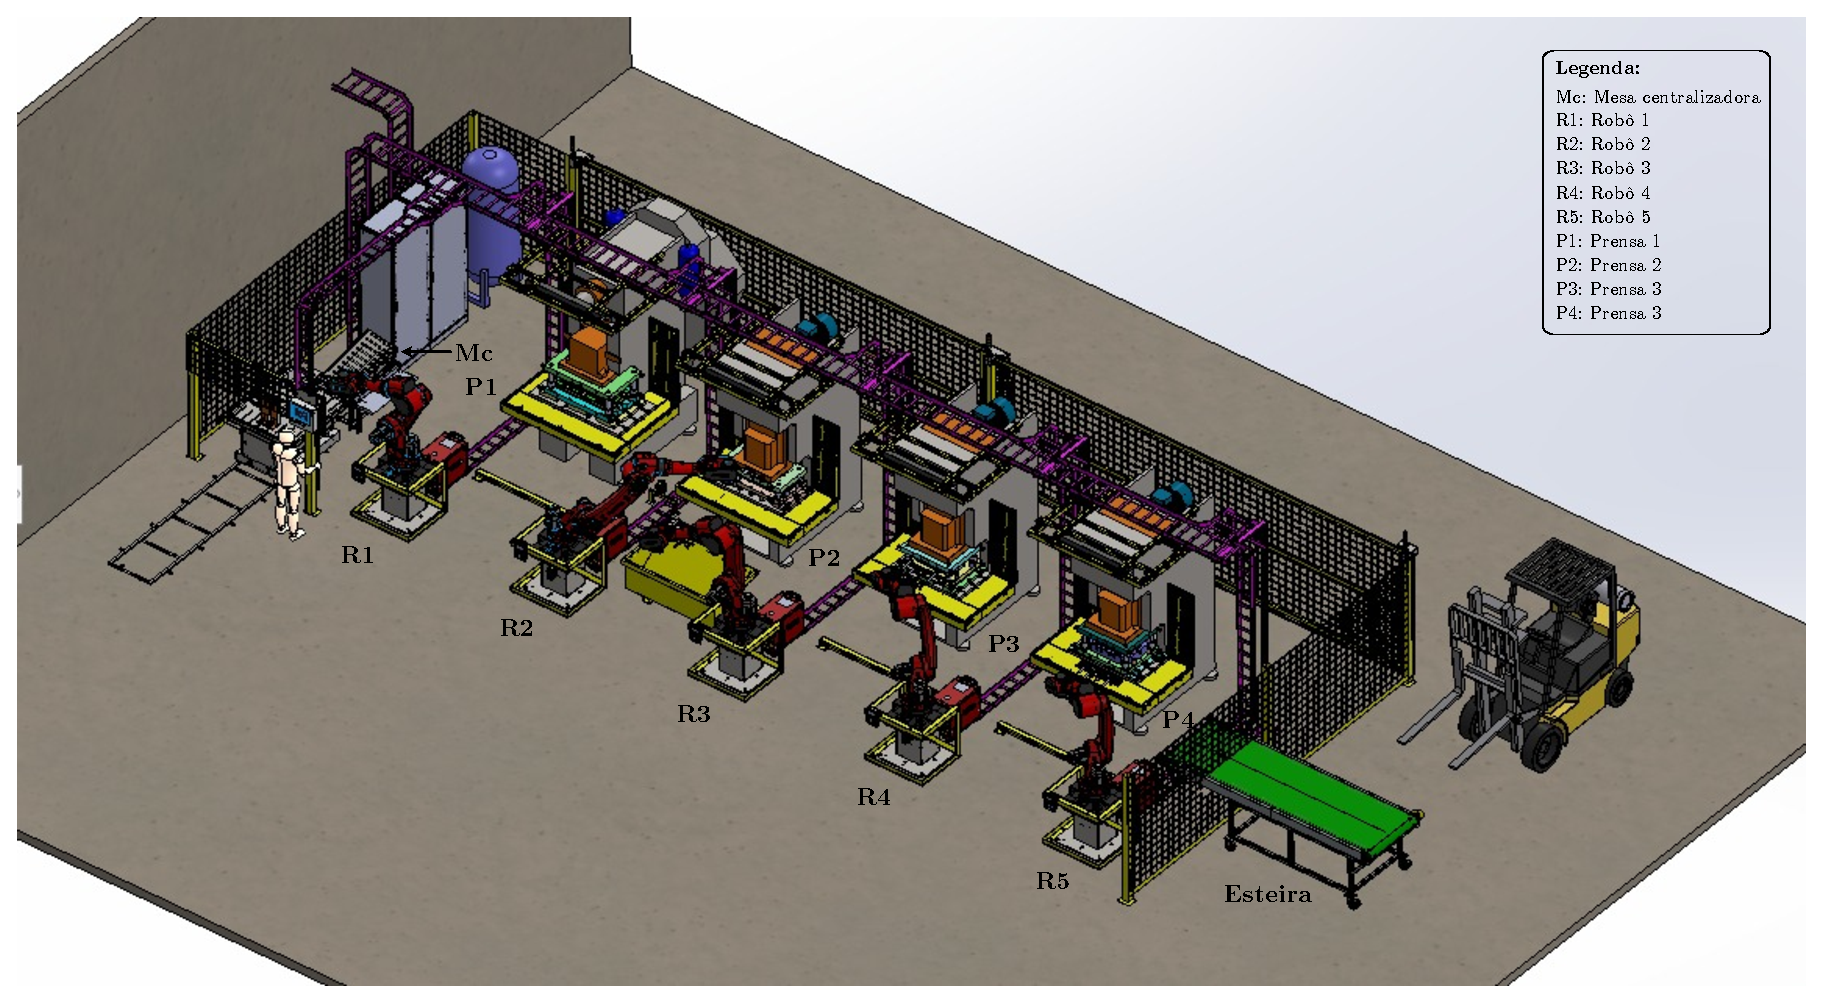
\includegraphics[width=0.8\textwidth]{imagens/processo.eps}
    \caption{Planta industrial}\label{fig:processo}
\end{figure}

\subsection{Modelos das Plantas}
Robô 1
\begin{figure}[H]%
    \centering
    \includegraphics[width=0.9\textwidth]{imagens/robo_1.eps}
    \caption{Planta Robô 1}\label{fig:robo1}
\end{figure}

Robô 2
\begin{figure}[H]%
    \centering
    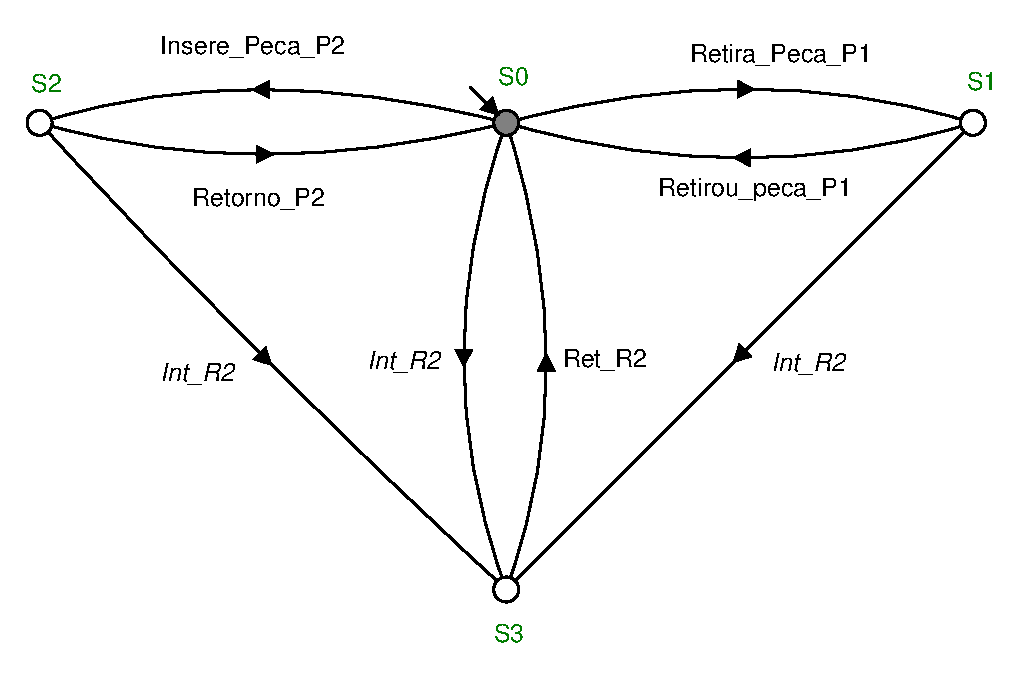
\includegraphics[width=0.9\textwidth]{imagens/robo_2.eps}
    \caption{Planta Robô 2}\label{fig:robo2}
\end{figure}

Robô 3
\begin{figure}[H]%
    \centering
    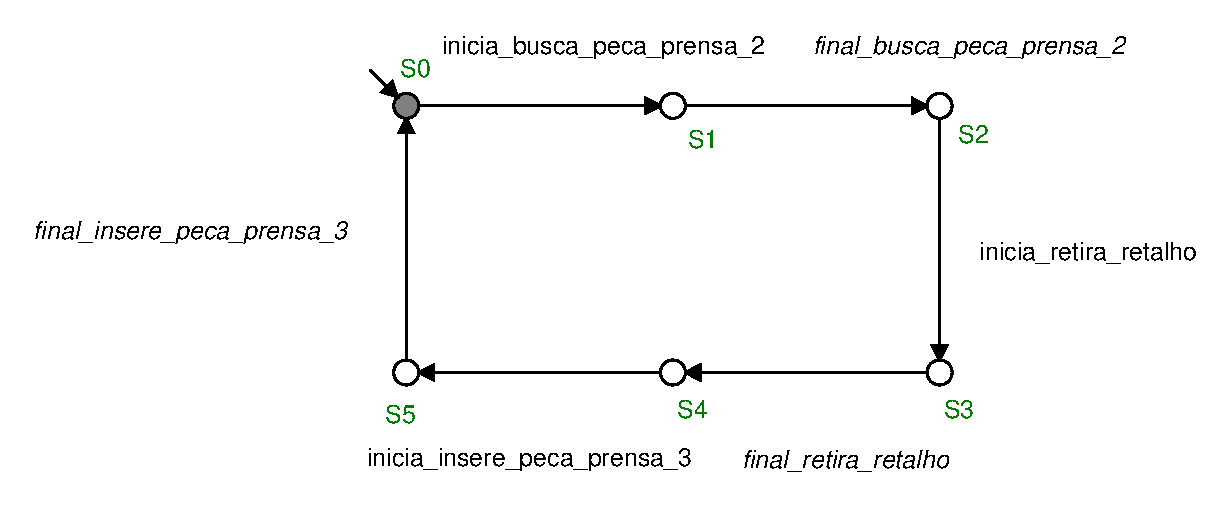
\includegraphics[width=0.9\textwidth]{imagens/robo_3.eps}
    \caption{Planta Robô 3}\label{fig:robo3}
\end{figure}

Robô 4
\begin{figure}[H]%
    \centering
    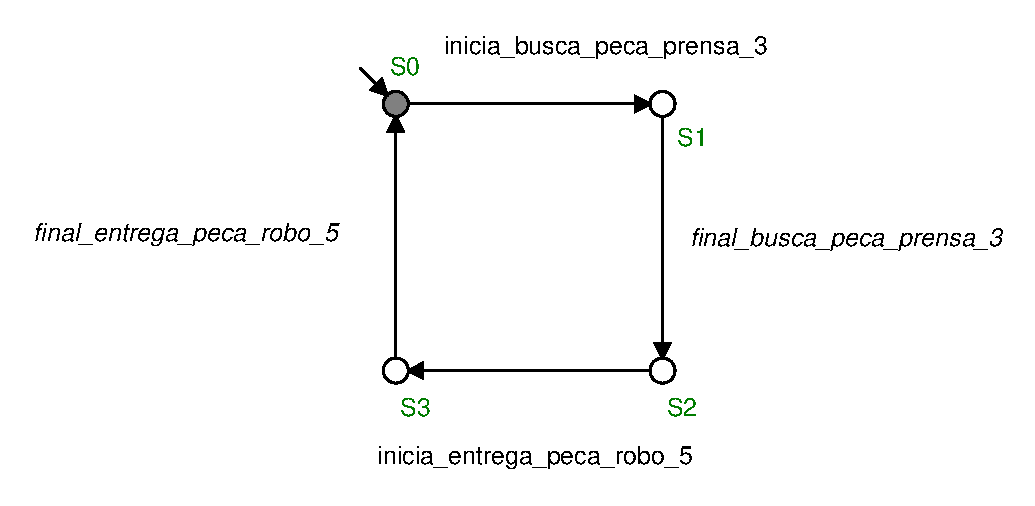
\includegraphics[width=0.9\textwidth]{imagens/robo_4.eps}
    \caption{Planta Robô 4}\label{fig:robo4}
\end{figure}

Robô 5
\begin{figure}[H]%
    \centering
    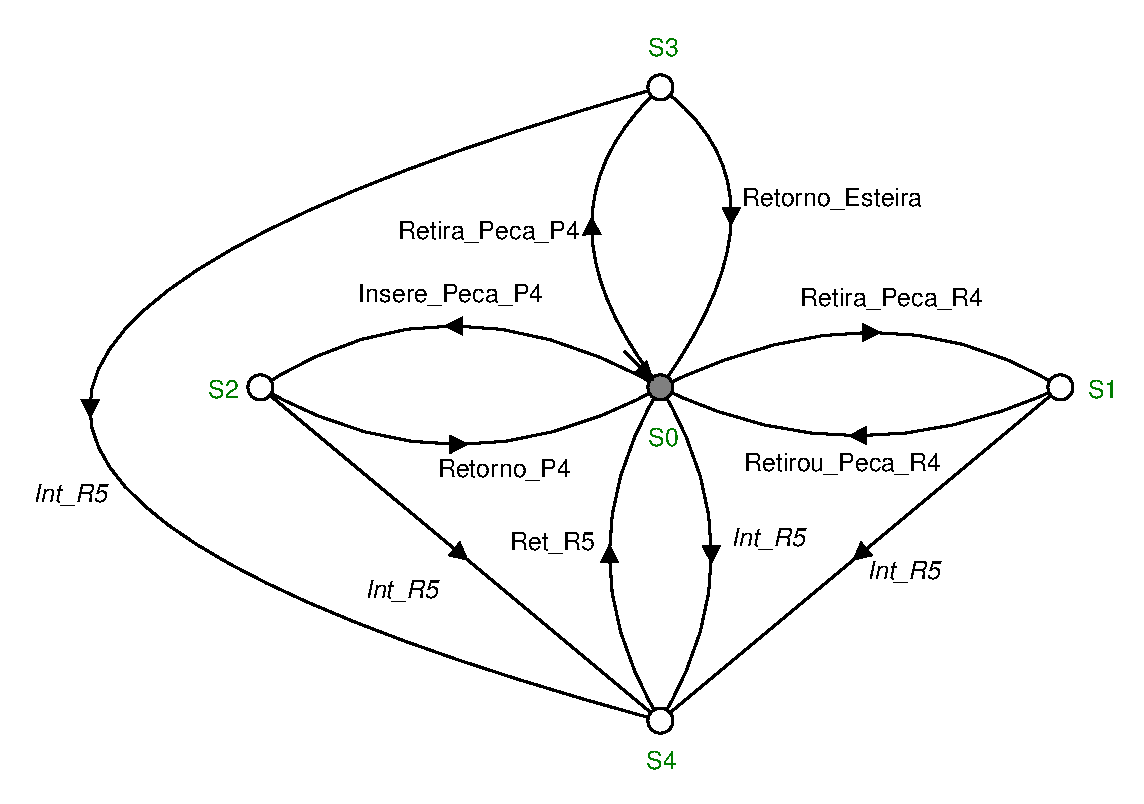
\includegraphics[width=0.9\textwidth]{imagens/robo_5.eps}
    \caption{Planta Robô 5}\label{fig:robo5}
\end{figure}

Mesa centralizadora
\begin{figure}[H]%
    \centering
    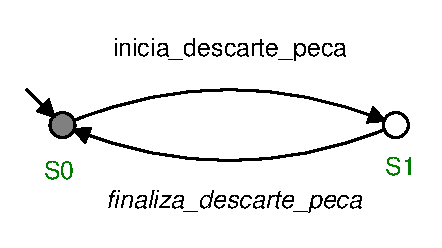
\includegraphics[width=0.9\textwidth]{imagens/mesa_centralizadora.eps}
    \caption{Planta Mesa centralizadora}\label{fig:mesa}
\end{figure}

Todas as prensas têm o mesmo modelo, a seguir é apresentado o modelo da prensa 1.
\begin{figure}[H]%
    \centering
    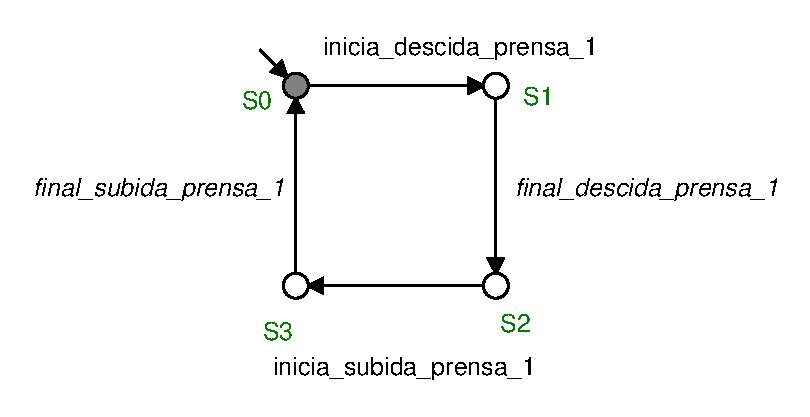
\includegraphics[width=0.9\textwidth]{imagens/prensa_1.eps}
    \caption{Planta Prensa}\label{fig:prensa}
\end{figure}

Sensor chapa dupla
\begin{figure}[H]%
    \centering
    
\includegraphics[width=0.9\textwidth]{imagens/sensor_chapa_dupla.eps}
    \caption{Sensor chapas duplas}\label{fig:chapadupla}
\end{figure}

Todos os bimanuais de liberação das prensas tem o mesmo modelo, a seguir é apresentado o modelo bimanual da prensa 1.
\begin{figure}[H]%
    \centering
    
\includegraphics[width=0.9\textwidth]{imagens/bimanual_prensa_1.eps}
    \caption{Sensor Bimanual}\label{fig:bimanual}
\end{figure}

\section{Modelos das Especificações}
Especificação 1 direciona a mesa centralizadora e robô 1 com base no sensor de chapas duplas.
\begin{figure}[H]%
    \centering
    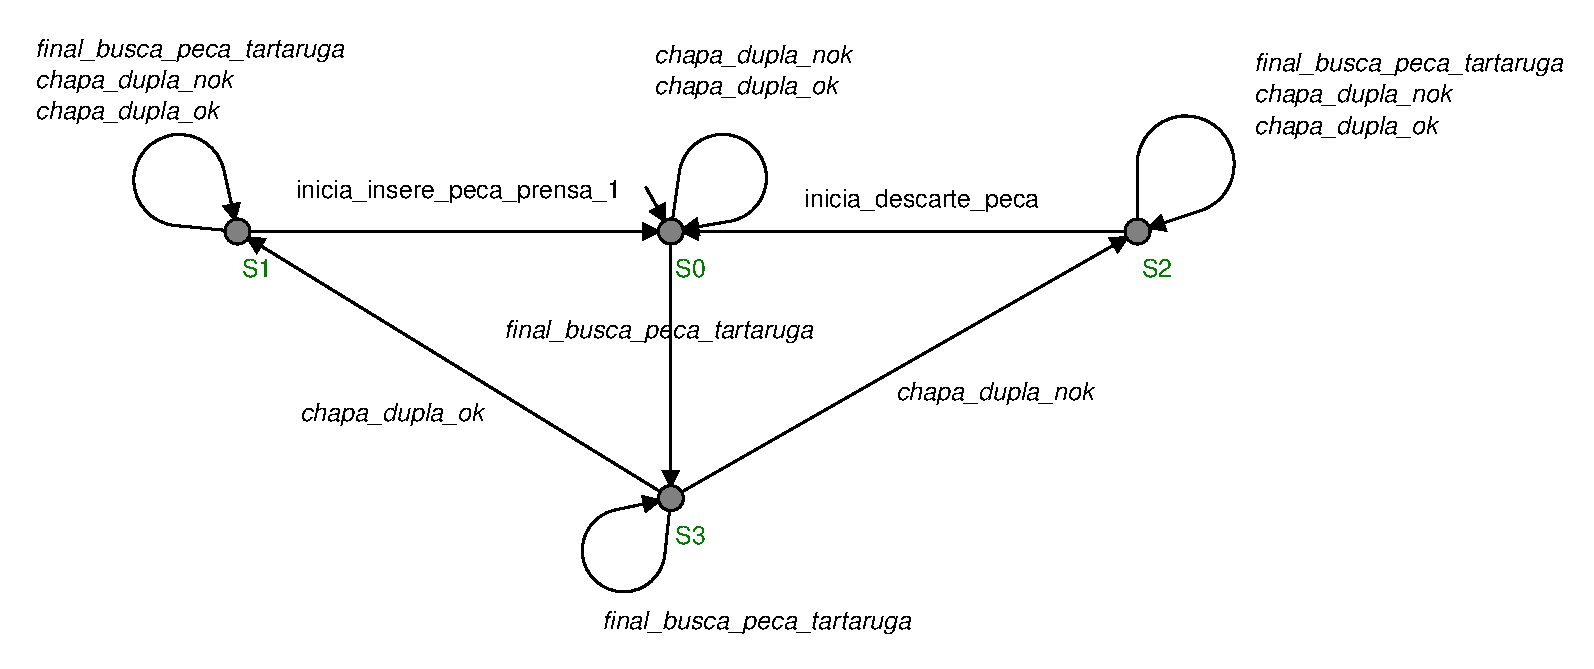
\includegraphics[width=0.9\textwidth]{imagens/E1_decide_chapa_dupla.eps}
    \caption{Especificação para descarte chapa dupla}\label{fig:especificacao1}
\end{figure}

\section{Solução de controle}
Estrutura modular Especificação 2
\begin{figure}[H]%
    \centering
    \includegraphics[width=0.9\textwidth]{imagens/Modular_structure.eps}
    \caption{Modularização}\label{fig:modular}
\end{figure}